\documentclass{article}
\usepackage{amsmath}
\usepackage{graphicx}
\usepackage{float}
\usepackage[utf8]{inputenc}

\usepackage{pythonhighlight}




\title{MTH 5315 NUMERICAL METHODS FOR PDE \\ 
HOMEWORK 2 REPORT }

\date{Thursday 8th February 2018}
\author{Max Le ID:901223283}


\begin{document}
	
	\maketitle
	\newpage
	
	\section{PART 1}
	
	We have the following problem:
	\begin{align*}
	u_t - u_x = 0 \\ 
	x \in [0, 1]
	\end{align*}
	\noindent
	With prescribed initial condition and periodic boundary conditions for the scheme: 
	
	\begin{equation}
	\frac{U_{j}^{k+1} - 0.5(U_{j+1}^{k}+U_{j-1}^{k})}{\Delta t}- \frac{U_{j+1}^{k}-U_{j-1}^{k}}{2\Delta x} = 0
	\end{equation}
	

	
	
	\subsection{For dt = 0.5dx}
	
	\subsubsection{1st initial condition}
	
	\begin{equation*}
	u(x,0) = sin(4\pi x)
	\end{equation*}
	
	\begin{figure}[H]
		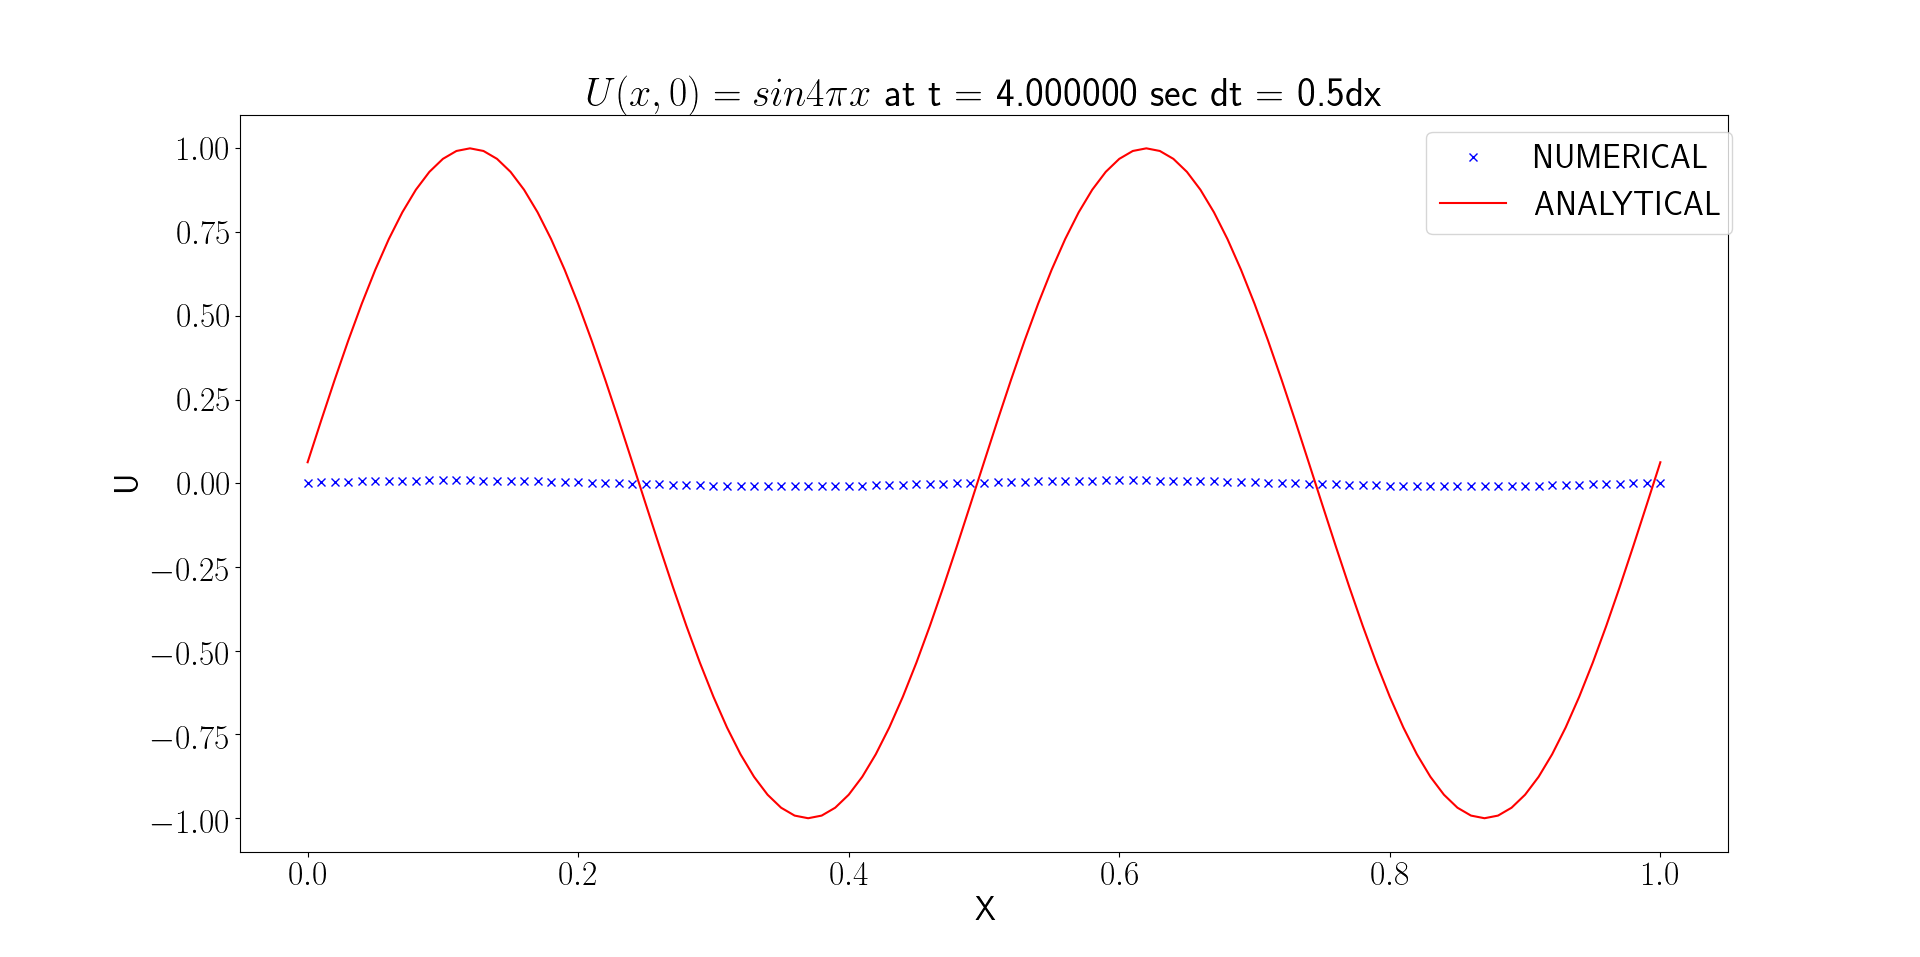
\includegraphics[width=\linewidth]{plot_1A.png}
		\caption{Numerical vs Analytical at t = 4 seconds for 1st IC, dt = 0.5dx}
		
	\end{figure}
	\noindent
	Observation: The numerical solution's amplitude dissipates as time goes to 4 seconds.  We can see visually that the solution lost approximately 90\% of its amplitude.  In the code, this is computed as follow: 
	
	\begin{equation}
	\% damping = 100*\left(1-\frac{max(numerical)- min(numerical)}{max(analytical)-min(analytical)}\right)
	\end{equation}
	\noindent
	The is calculated to be around 99.13\%.  This makes sense because we can see that the solution loses most of its amplitudes.
	
	
	\begin{figure}[H]
		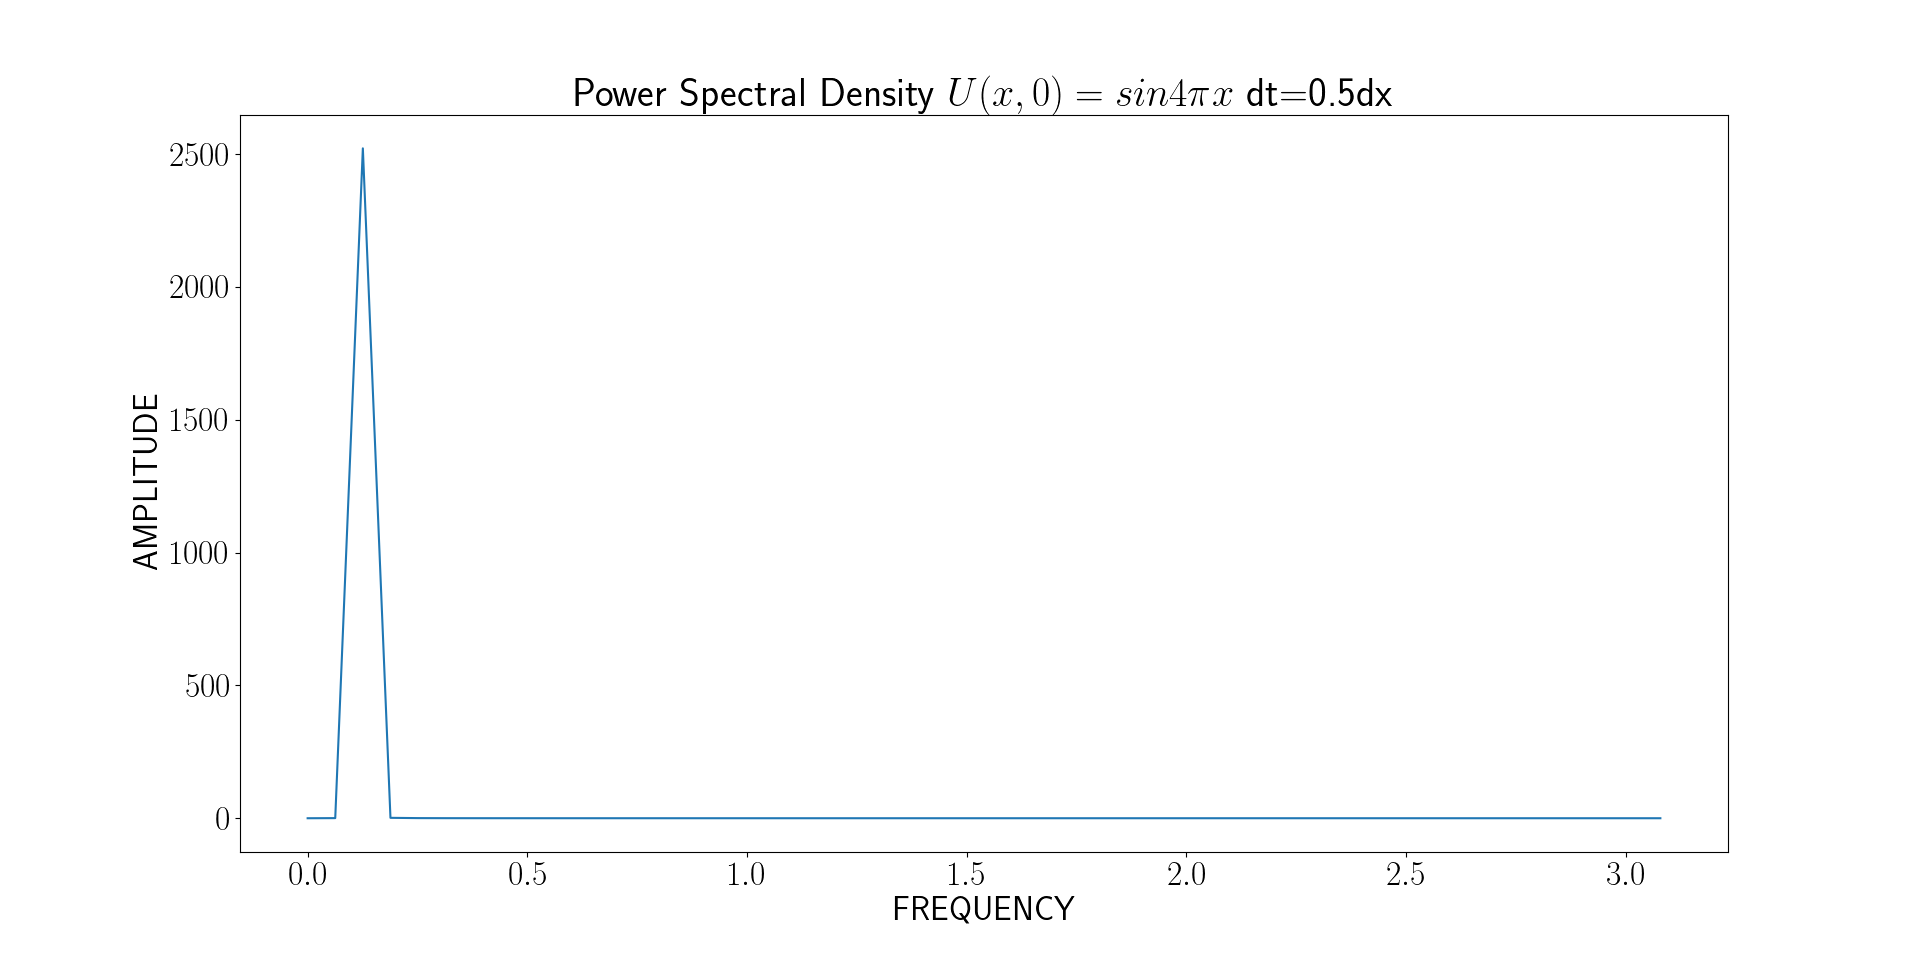
\includegraphics[width=\linewidth]{power_spectral_1A.png}
		\caption{Power spectral density for 1st IC, dt = 0.5dx}
		
	\end{figure}
	\noindent
	Observation: For this power spectral density plot, we see that there is only 1 peak. This peak is the wave number, or $4\pi$.  The frequency that this occurs is, $4\pi \Delta x \approx 0.125$. In the code, this is calculated by looking at the maximum value on the power spectral density plot, or fmax in the code. 
	
	
	\subsubsection{2nd initial condition}
	
	\begin{equation*}
	u(x,0) = sin^{10}(2 \pi x)
	\end{equation*}
	
	
	\begin{figure}[H]
	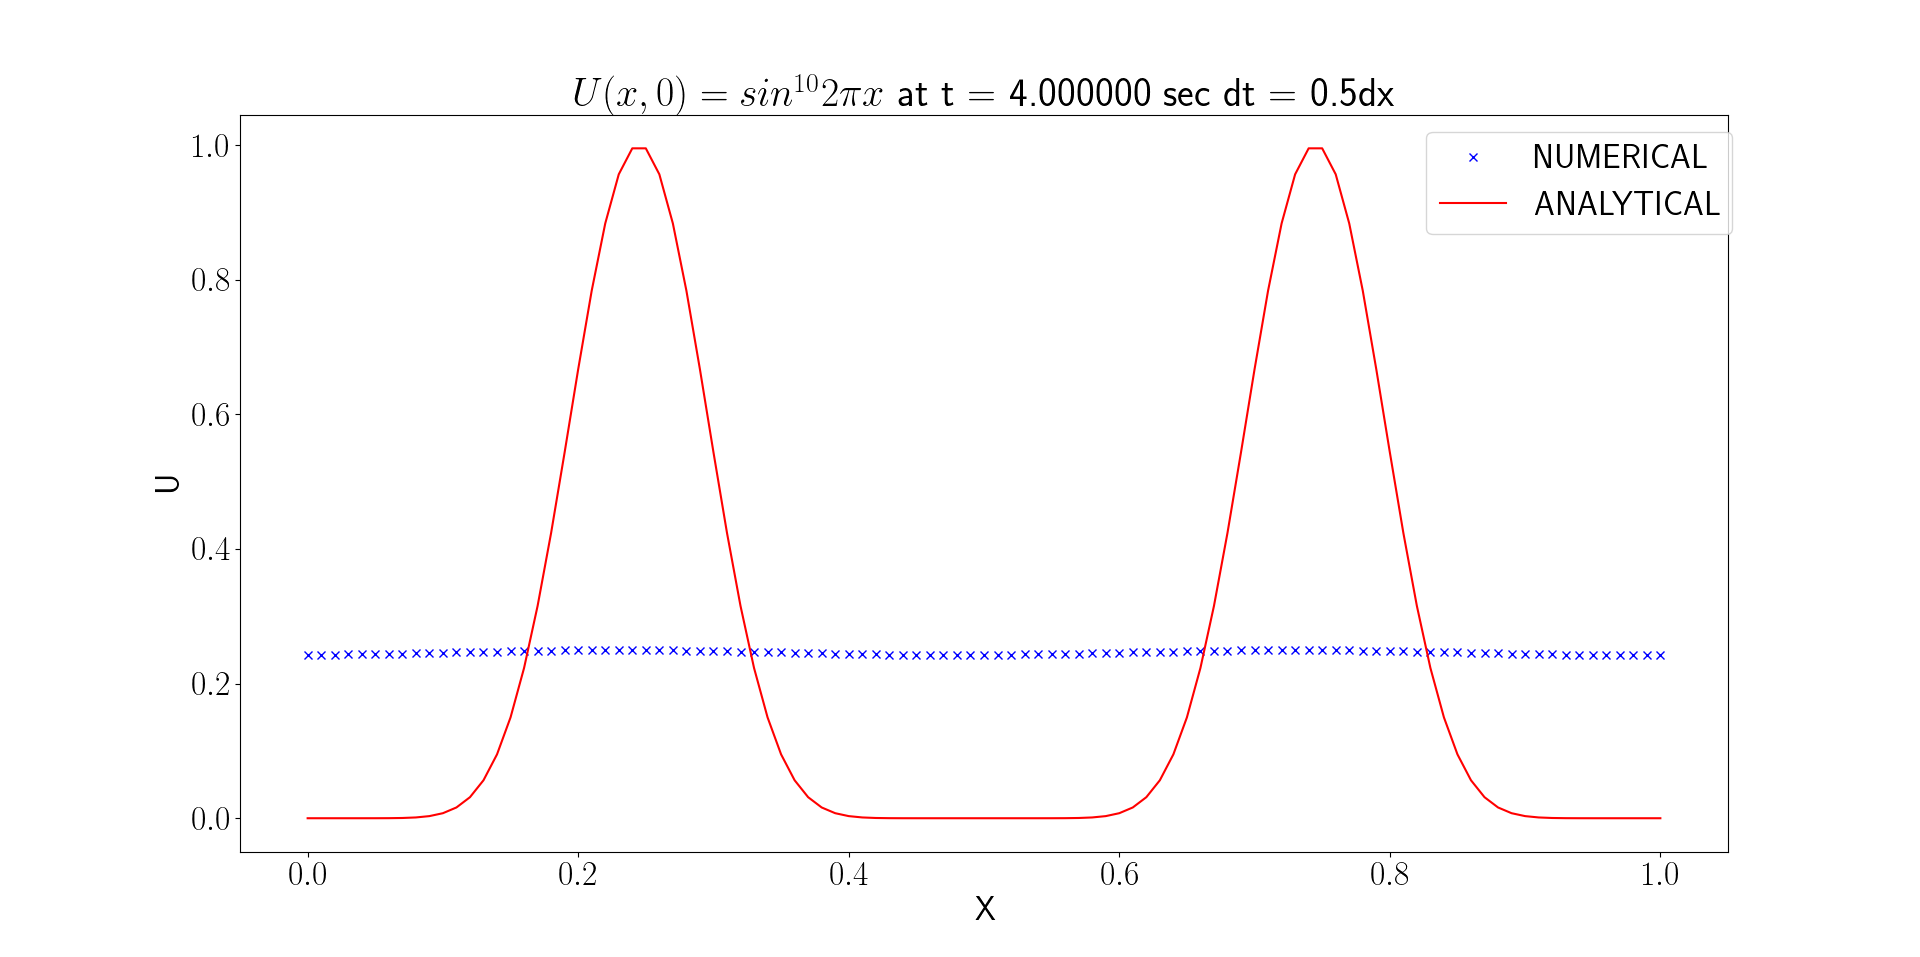
\includegraphics[width=\linewidth]{plot_1B.png}
	\caption{Numerical vs Analytical at t = 4 seconds for 2nd IC, dt = 0.5dx}
		
	\end{figure}
	\noindent
	Observation: This numerical solution still dissipates as time goes to 4 seconds.  Although, this time the solution does not go to 0, but it fluctuates between 0.2 and 0.4. Using the similar formula to calculate the percentage damping as above, we see that the computer gives 99.28\% damping
	
	\begin{figure}[H]
		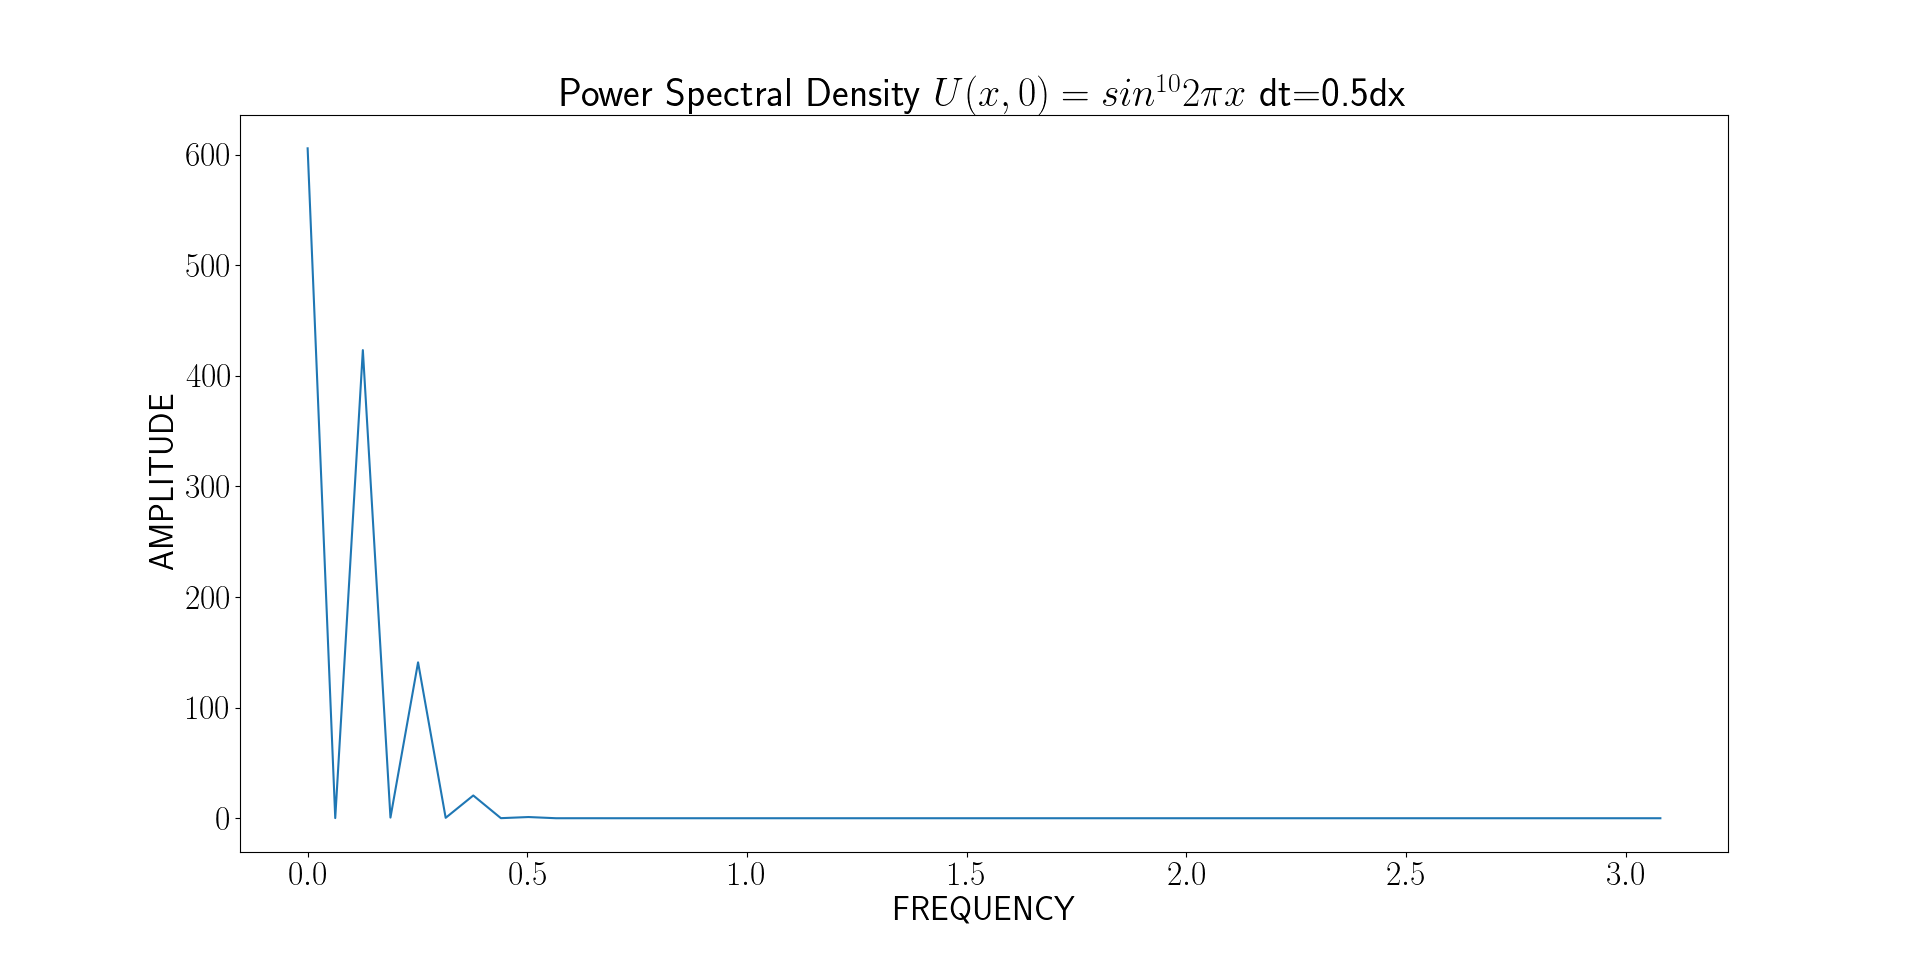
\includegraphics[width=\linewidth]{power_spectral_1B.png}
		\caption{Power spectral density for 2nd IC, dt = 0.5dx}
		
	\end{figure}
	\noindent
	Observation: The power spectral density plot has multiple peaks. This could be due to numerical errors.  The max peak should occur at $2\pi$ or frequency of $2\pi \Delta x \approx 0.06$. The computer gives 0 as the answer for this max peak. The reason for this could be due to numerical inaccuracy,that there is not enough points to resolve the maximum peak. Upon closer inspection, we can see that there are jagged lines in the numerical solution, which is difficult for the program to determine which one is the maximum peak.  
	
	
	
	
	
	
	
	
	\newpage
	\subsection{For dt = dx}
	\subsubsection{1st initial condition}
	
	\begin{equation*}
	u(x,0) = sin(4\pi x)
	\end{equation*}
	
	
	\begin{figure}[H]
	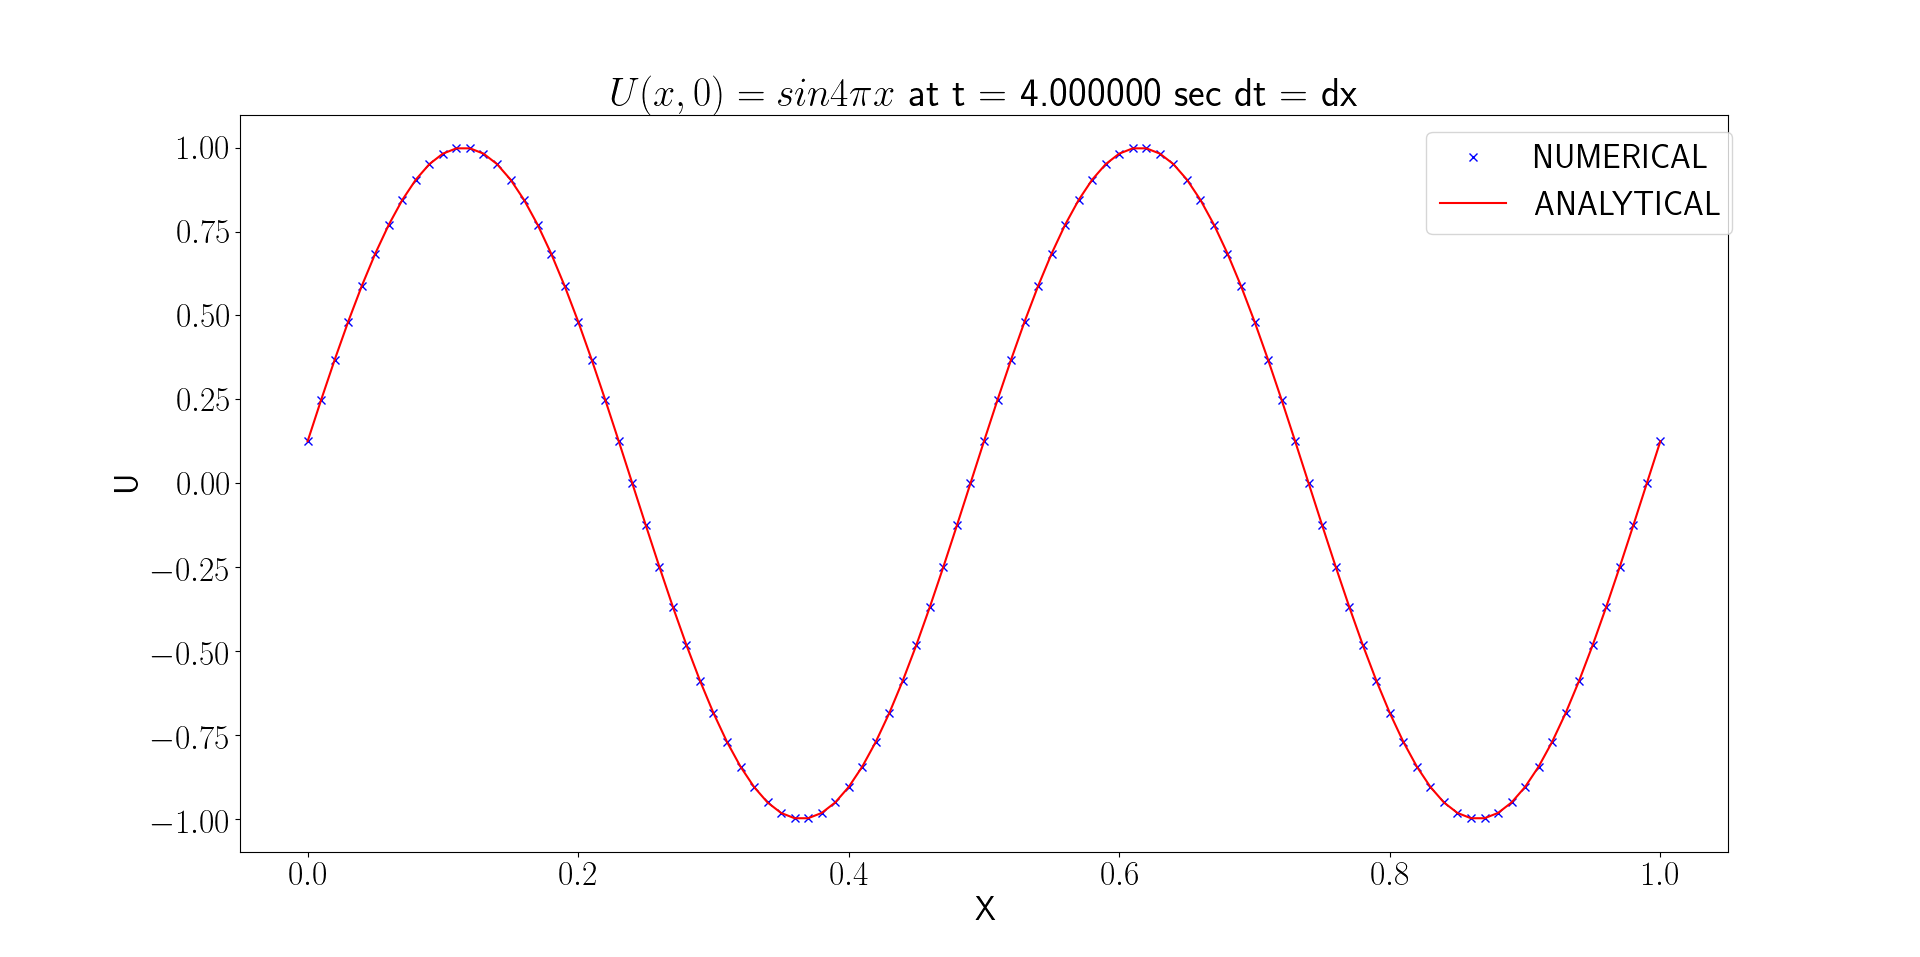
\includegraphics[width=\linewidth]{plot_1C_FIRST.png}
	\caption{Numerical vs Analytical at t = 4 seconds for 1st IC, dt = dx}
		
	\end{figure}
	\noindent
	Observation: As dt = dx, or as we reach the maximum CFL condition, the numerical solution is exactly the analytical one and does not dissipate. Moreover, when the value of damping is computed, the code returns 0.0 as the answer.  This makes sense because there are no damping.  
	
	\begin{figure}[H]
	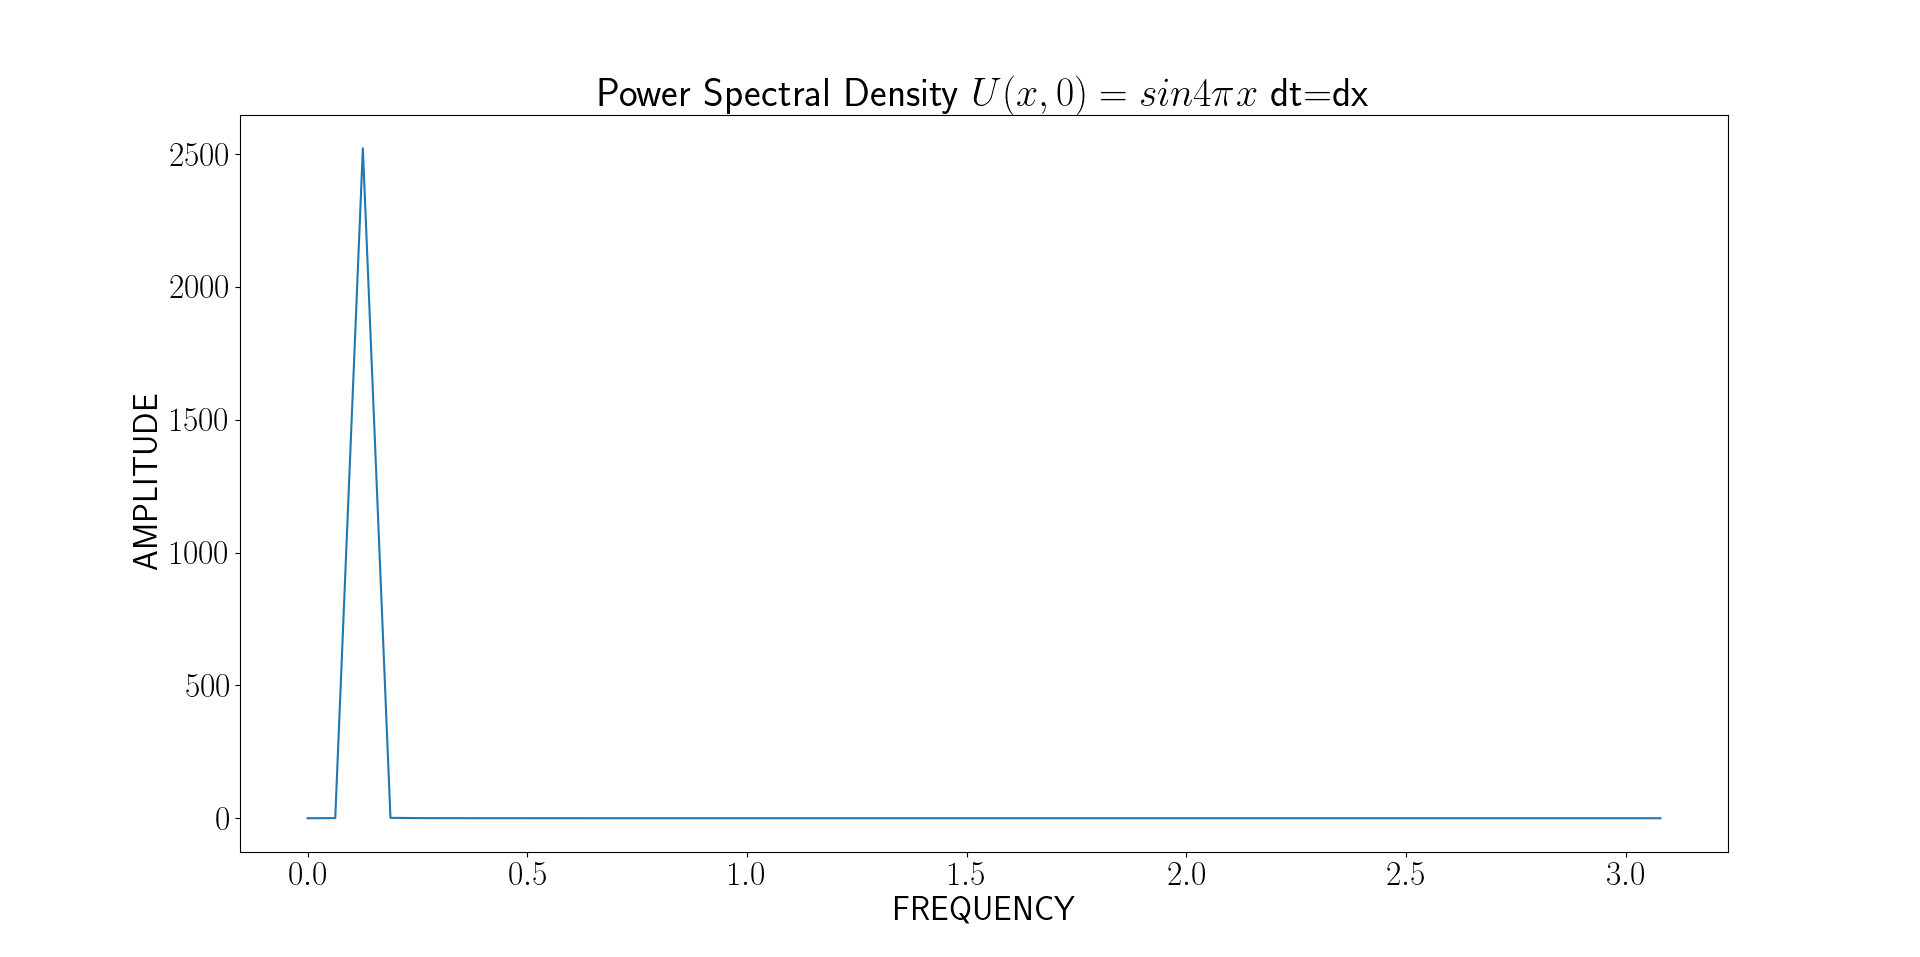
\includegraphics[width=\linewidth]{power_spectral_1C_FIRST.png}
	\caption{Power spectral density for 1st IC, dt = dx}
		
	\end{figure}
	\noindent
	Observation: We use the same initial condition, with only changes in the CFL condition.  Therefore, the peak on the power spectral density should stay be the same, which it is. This is because the nature of the equation is the same, but the rate of convergence changes.   


	\subsubsection{2nd initial condition}
	
	\begin{equation*}
	u(x,0) = sin^{10}(2 \pi x)
	\end{equation*}
	
	\begin{figure}[H]
	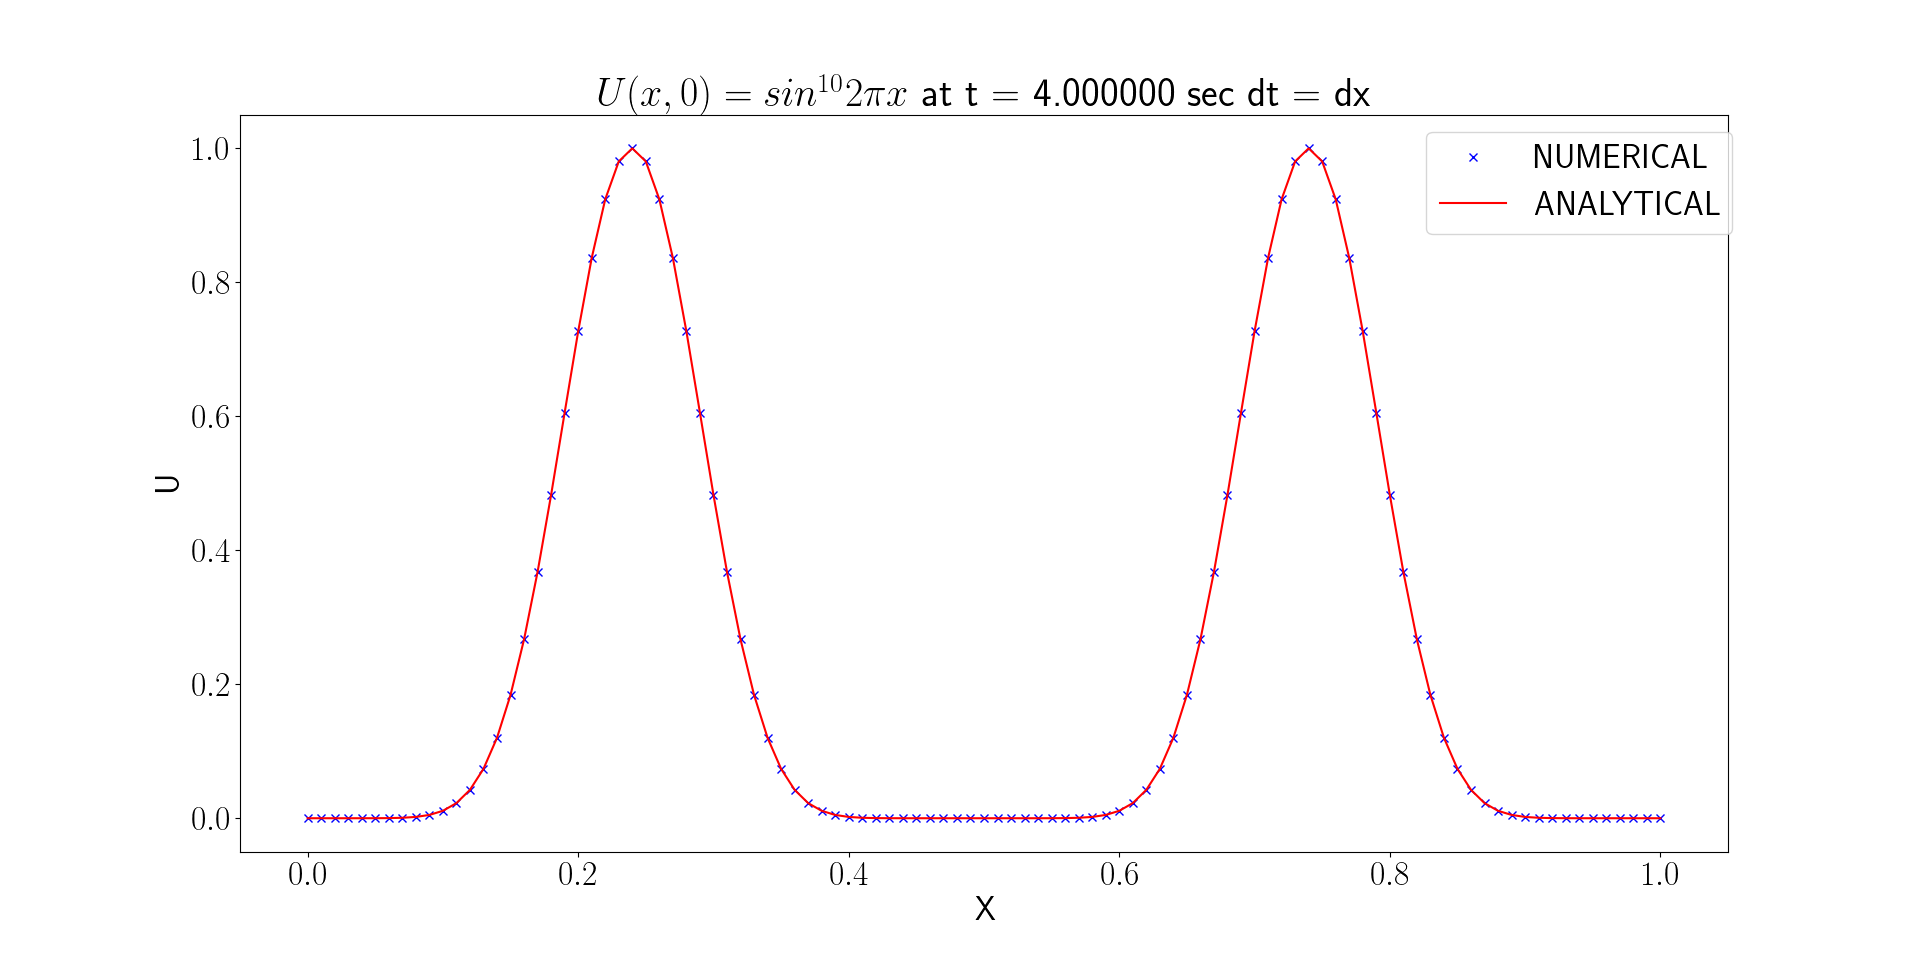
\includegraphics[width=\linewidth]{plot_1C_SECOND.png}
	\caption{Numerical vs Analytical at t = 4 seconds for 2nd IC,dt = dx}
		
	\end{figure}
	\noindent
	Observation: Similar to the previous part, max CFL condition guarantees convergence and we can see that the numerical solution matches the analytical one perfectly. As expected, when the value for damping is computed, the computer returns 0 as the answer (no damping, exact solution) 
	
	\begin{figure}[H]
	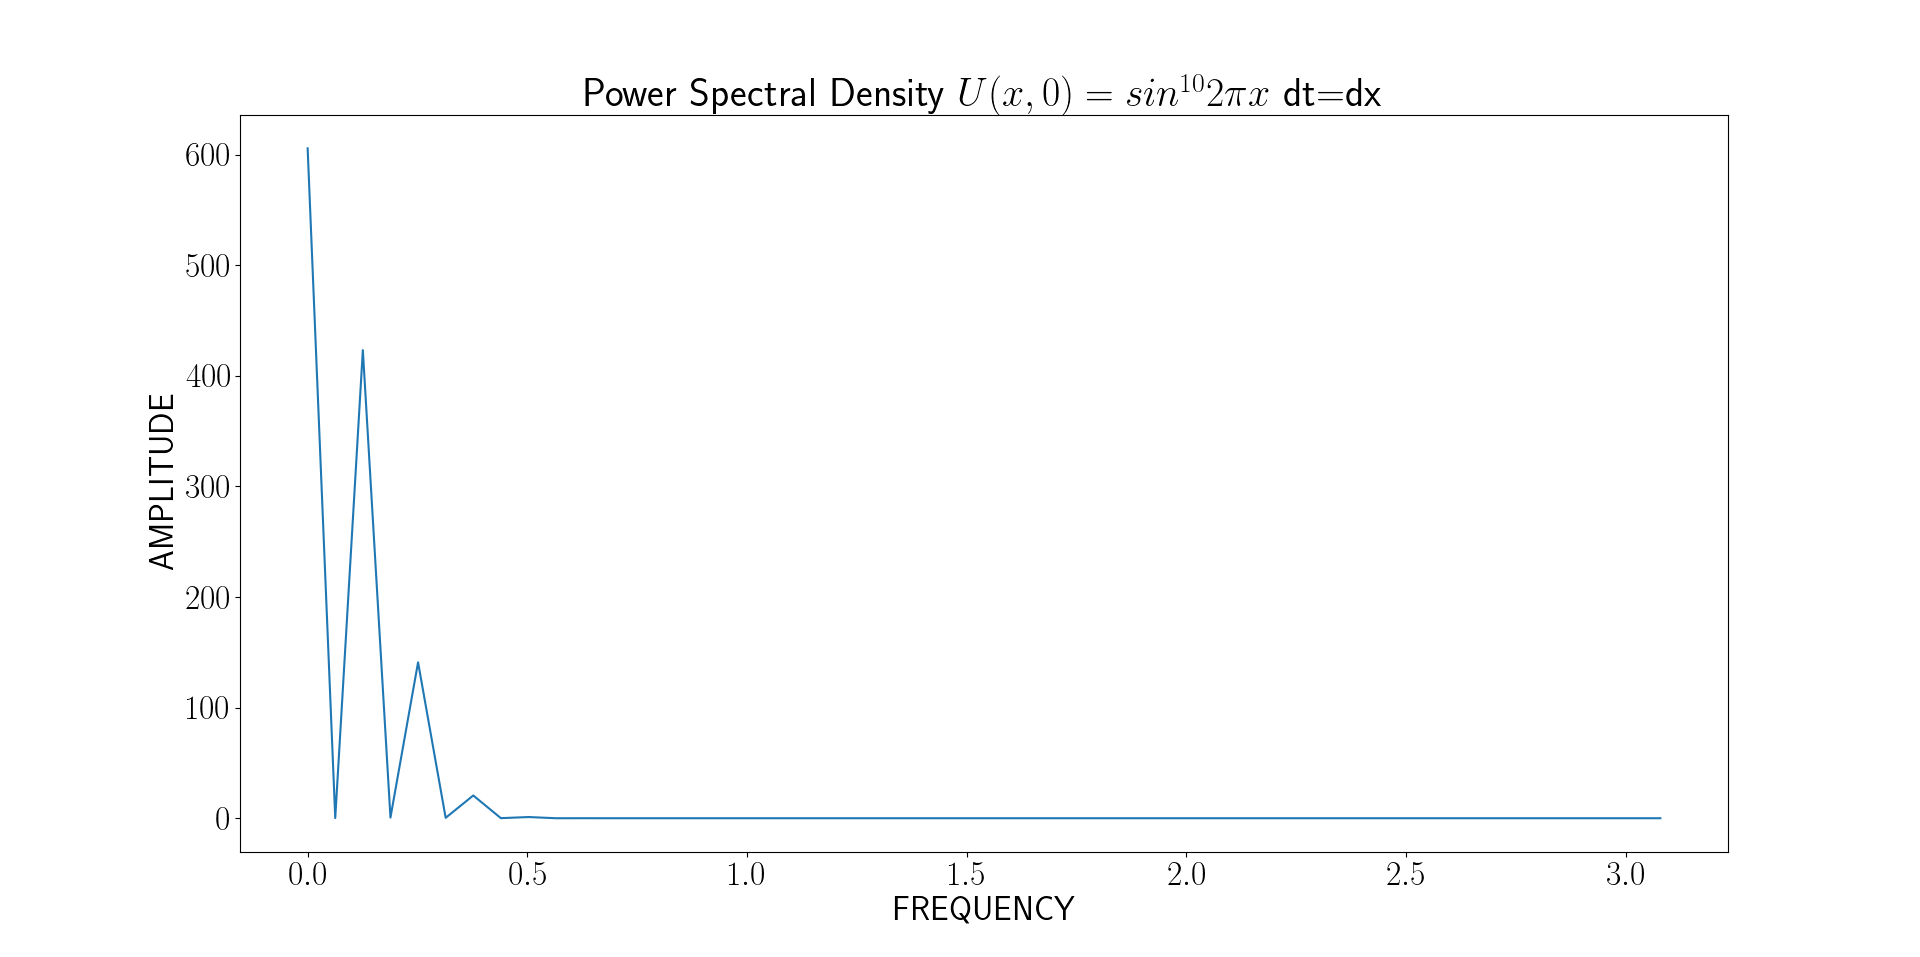
\includegraphics[width=\linewidth]{power_spectral_1C_SECOND.png}
	\caption{Power spectral density for 2nd IC, dt = dx}
		
	\end{figure}
	\noindent
	Observation: Again, we only change the CFL conditions, so the peak of the power spectral density should be similar to when dt = 0.5dx.  

	

	
	\newpage
	
	\section{PART 2}
	
	We have the following problem: 
	
	\begin{align*}
	u_t + au_x = 0\\
	R = \frac{\Delta t}{\Delta x}
	\end{align*}
	\noindent
	For the following scheme: 
	
	\begin{equation}
	u_{j}^{k+1}+\frac{R}{4}(U_{j+1}^{k+1}-U_{j-1}^{k+1}) = U_{j}^{k}-\frac{R}{4}(U_{j+1}^{k}-U_{j-1}^{k})
	\end{equation}
	
	
	
	\subsection{Analyze dissipative and dispersive qualities of the scheme}
	
	We start by substituting the following Fourier mode into our numerical scheme: 
	
	\begin{equation}
	u_{j}^{k} =  \hat{u} e^{i(\alpha+ib)k\Delta t}e^{i\beta j \Delta x}
	\end{equation}
	
	
	\noindent	
	After dividing by common $\hat{u}$ expression.  We get:
	
	\begin{equation*}
	e^{i(\alpha+ib)\Delta t} = 1- \dfrac{R}{4}(e^{i\beta\Delta x}-e^{-i\beta\Delta x})- \dfrac{R}{4}(e^{i(a+ib)\Delta t}e^{i\beta\Delta x}-e^{i(a+ib)\Delta t}e^{-i\beta\Delta x})
	\end{equation*}
	
	
	
	\noindent
	Letting $\beta \Delta x = \theta$. Collecting terms, isolating the exponential terms on one side and simplifying, we get: 
	
	\noindent
	In other words:
	\begin{equation*}
	e^{i(a+ib)\Delta t} + e^{i(a+ib)\Delta t}\dfrac{R}{4}\left( e^{i\theta} - e^{-i\theta} \right) = 1-\dfrac{R}{4}\left( e^{i\theta} - e^{-i\theta} \right)
	\end{equation*}
	
	\begin{equation*}	
	e^{-b \Delta t}e^{i \alpha \Delta t} = \dfrac{1-\dfrac{R}{4}(e^{i \theta}-e^{-i \theta})}   {1+\dfrac{R}{4}(e^{i \theta}-e^{-i \theta})}
	\end{equation*}
	
	\noindent
	For dissipation, we want the norm of the RHS for $e^{-b \Delta t}$
	
	\begin{equation*}
	\begin{aligned}
	\left|e^{-b \Delta t}\right |^2 &= \left|   \dfrac{1-\dfrac{R}{4}(e^{i \theta}-e^{-i \theta})}   {1+\dfrac{R}{4}(e^{i \theta}-e^{-i \theta})}  \right |^2	\\ &= \left|   \dfrac{1-\dfrac{R}{2}(isin \theta )}   {1+\dfrac{R}{2}(isin\theta)}  \right | ^2 \\&=\left|   \dfrac{1-\dfrac{R}{2}(isin \theta )}   {1+\dfrac{R}{2}(isin\theta)}   * \dfrac{1-\dfrac{R}{2}(isin \theta )}   {1-\dfrac{R}{2}(isin\theta)} \right | ^2 
	\end{aligned}
	\end{equation*}
	\noindent
	Simplifying, splitting into real and imaginary parts 
	
	
	\begin{equation*}
	\begin{aligned}
		\left|e^{-b \Delta t}\right|^2 &= \left(\dfrac{1-\dfrac{R^2}{4}\sin^{2}\theta} {1+\dfrac{R^2}{4}\sin^{2}\theta}\right)^2 +\left(\dfrac{iR\sin\theta} {1+\dfrac{R^2}{4}\sin^{2}\theta}\right)^2 \\ 
		&= \dfrac{1}{1+\dfrac{R^2}{4}\sin \theta } * \left[1+ \dfrac{R^2}{2}\sin^{2} \theta + \dfrac{R^4}{16}\sin^{4} \theta      \right] \\
		&= \dfrac{\dfrac{1}{16}\left[16 + 8R^2\sin^2\theta + R^4 sin^4 \theta\right]}{\left(\dfrac{1}{4} (4+R^2\sin^2\theta)  \right)^2} \\ &= \dfrac{\left (R^2\sin^2\theta + 4 \right)^{2}}{\left (R^2\sin^2\theta + 4 \right)^{2}} \\ &= 1
	\end{aligned}
	\end{equation*} 
	\noindent
	This implies that $e^{-b\Delta t}$, or the damping factor, is a constant. Or we can also say that this scheme has no dissipations, because the new amplitude is 1* old amplitude, or no change in amplitude. 
	
	\noindent
	For dispersive, we need: 
	
	\begin{equation*}
	\begin{aligned}	
	tan(\alpha \Delta t) &= \dfrac{Imaginary}{Real}\\ &= \dfrac{-R\sin\theta}{1-\dfrac{R^2}{4}sin^2\theta}\\ &= \dfrac{-4R\sin\theta}{4-sin^2\theta}
	\end{aligned}
	\end{equation*}
	\noindent
	Solving for $\alpha \Delta t$, we get:
	
	\begin{equation*}
	\alpha \Delta t= \arctan\left( \dfrac{-4Rsin\theta}{4-R^2\sin^2\theta}\right)
	\end{equation*}
	
	
	\noindent
	Recall the following Taylor series expansions, at $x = 0$:
	
	\begin{equation*}
	sin(x) = x - \dfrac{x^3}{6}	+ \dfrac{x^5}{120} + ....
	\end{equation*}
	\begin{equation*}
	sin^2(x) = x^2 - \dfrac{x^4}{3}	+ \dfrac{2x^6}{45}-....
	\end{equation*}
	\begin{equation*}
	\arctan(x) = x - \dfrac{x^3}{3}	+ \dfrac{x^5}{5}+....
	\end{equation*}
	\begin{equation*}
	\dfrac{1}{1-ax^2} = 1 + ax^2 + a^2x^4
	\end{equation*}
	
	\noindent
	Substituting into the expression for $tan(\alpha \Delta t)$, neglecting higher order terms (bigger than $O(\Delta x^3 )$)
	
	\begin{equation*}
	\begin{aligned}
	tan(\alpha \Delta t) &= \dfrac{-4Rsin\theta}{4-R^2sin^2\theta}\\ &=-\dfrac{4R(\theta-\dfrac{\theta^3}{6})}{4-R^2(\theta^2)}\\&=\dfrac{4R\theta}{4-R^2\theta ^2} - \dfrac{4R\theta^3}{6(4-R^2\theta^2)}\\&=-R\theta\left( \dfrac{1}{1-\dfrac{R^2}{4}\theta^2}\right) - \dfrac{R\theta^3}{6}\left( \dfrac{1}{1-\dfrac{R^2}{4}\theta^2}\right)\\&=-R\theta\left(1+\dfrac{R^2}{4}\theta^2\right) - \dfrac{R\theta^3}{6}\left( 1+\dfrac{R^2}{4}\theta^2   \right) \\&=-R\theta + \dfrac{R^3\theta^3}{4} - \dfrac{R\theta^3}{6} + \text{Drop because higher order term}\\&=-R\theta + \dfrac{3R^3\theta^3}{12} - \dfrac{2R\theta^2}{12}\\&=-R\theta+\dfrac{\theta^3(3R^3-2R)}{12}\\&=-R\theta\left(  1+ \dfrac{\theta^2(3R^2-2)}{R}  \right)
	\end{aligned}
	\end{equation*}
	
	\noindent
	Now we substitute the series for $arctan(x)$:
	
	\begin{equation*}
	\begin{aligned}
	\alpha \Delta t &= -R\theta\left(1+ \dfrac{\theta^2(3R^2-2)}{R}  \right) - \dfrac{R^3\theta^3}{3}\left(1+ \dfrac{\theta^2(3R^2-2)}{R}\right)^3\\&=R\theta\left(1+ \dfrac{\theta^2(3R^2-2)}{R}  \right) - \dfrac{R^2\theta^2}{3} + \text{Drop higher order terms}\\&=-R\theta\left( 1+ \dfrac{\theta^2 (3R^2-2)}{12} - \dfrac{R^2\theta^2}{3}  \right)\\&=R\theta \left(  1+\theta^2\left(\dfrac{-4R^2+3R^2-2}{12} \right)\right)\\&=-R\theta\left( 1- \theta^2\left(\dfrac{R^2+2}{12} \right)  \right)
	\end{aligned}
	\end{equation*}
	
	\noindent
	Recall $R = \dfrac{a\Delta t}{\Delta x}$ and $\theta = \beta \Delta x$.  Substituting and solving for $\alpha$: 
	
	\begin{equation*}
	\alpha = -a\beta\left(1-\theta^2\left(\dfrac{R^2 + 2}{12}\right)\right)	
	\end{equation*}
	
	\noindent
	Recall numerical wave speed, $c = \dfrac{-\alpha}{\beta} $, we get: 
	
	\begin{equation}
	c = -a(1-\theta^2(R^2+2)\left(\frac{1}{12}\right)
	\end{equation}	
	
	
	\subsection{Plot the errors in the speed of propagation for Fourier Modes $0 \leq \beta \Delta x \leq \pi$}
	
	\noindent
	Given R = 0.5 and a = 1.0.  The following plot of the error in speed propagation is generated: 
	
	\begin{figure}[H]
	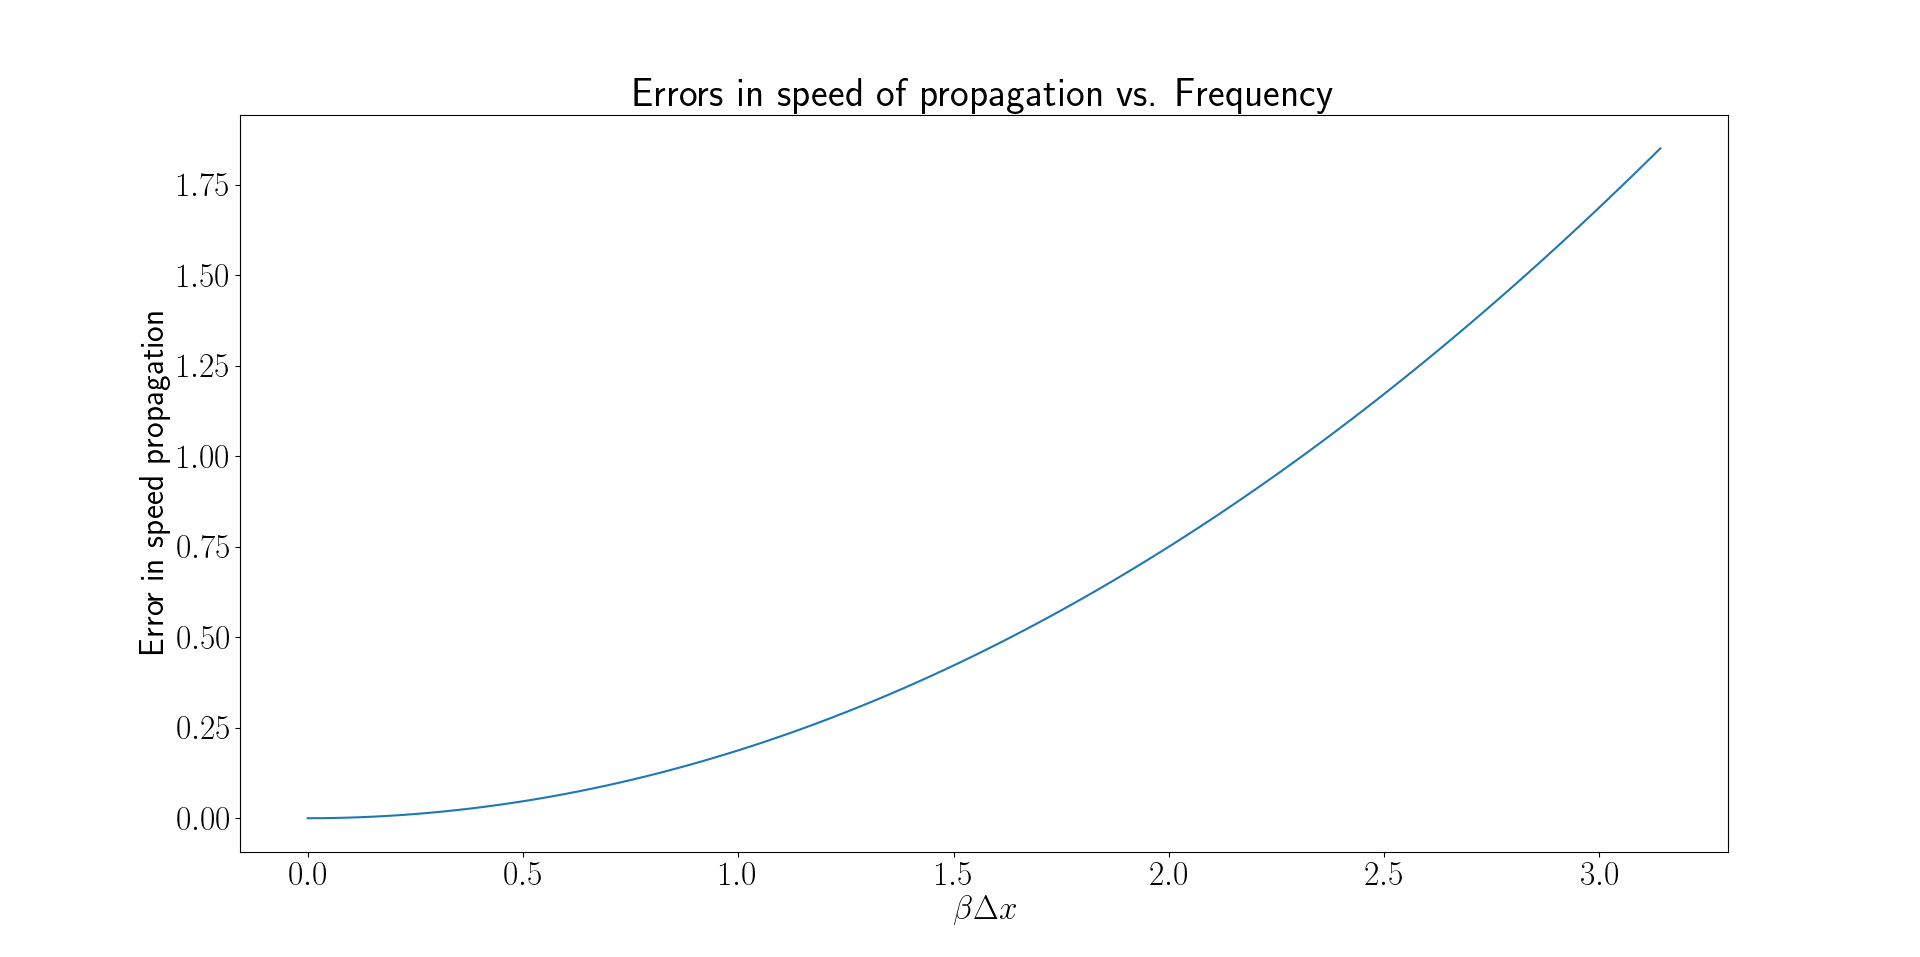
\includegraphics[width=\linewidth]{error_speed_05R.png}
	\caption{Error in speed of propagations for R = 0.5}		
		
	\end{figure}
	
	\noindent
	Observation: It can be seen that the error in speed of propagation increases with the frequency. Mathematically, the expression for the numerical wave speed involves a term: $R^2 + 2$ ,unlike examples in class, where R can be treated as less than or bigger than zero. We also have 1 - this quantity;therefore, the numerical wave speed is always slower than the analytical wave speed. We can say that this scheme is absolutely dispersive. 
	
	\begin{figure}[H]
	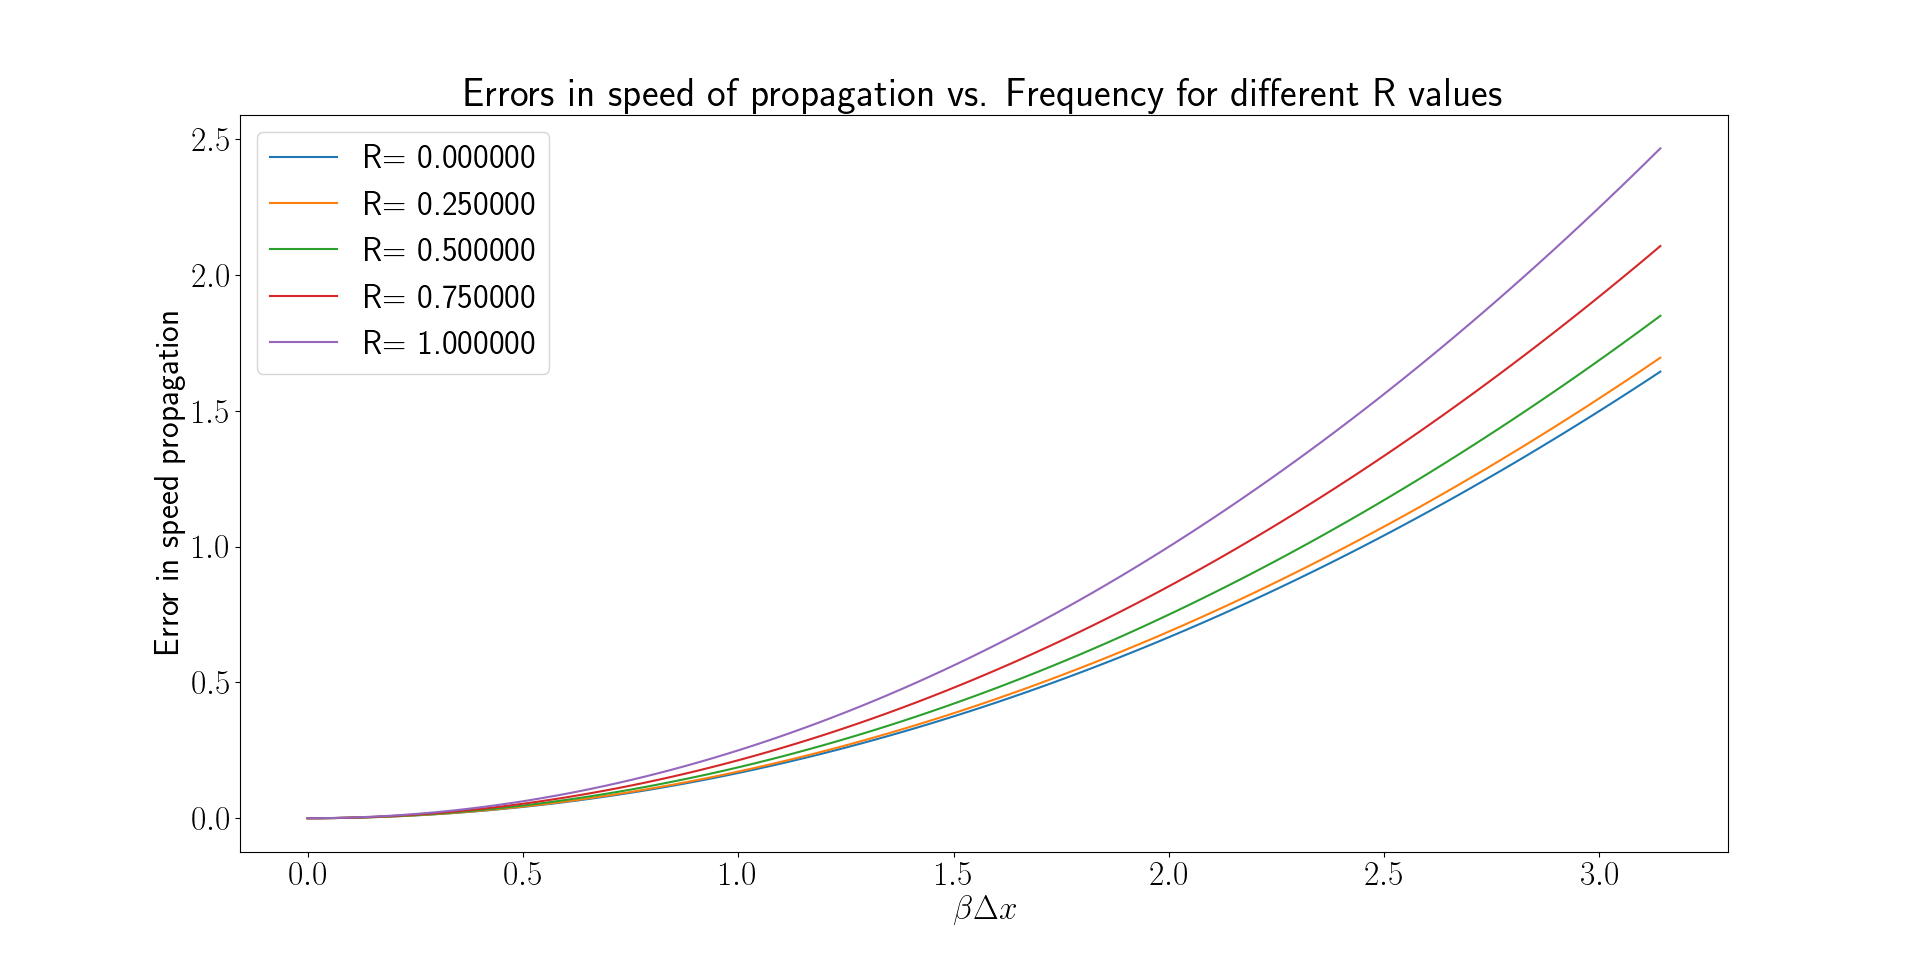
\includegraphics[width=\linewidth]{wave_test.png}
	\caption{Error in speed of propagations for different values of R}				
	\end{figure}

	\noindent
	In fact, when multiple values of R are tested, the plot shows the similar behavior: increasing error with increasing frequency.
	
	\newpage
	\section{PYTHON CODE}
	
	%\begin{python}
		
	\inputpython{mth5315_hw2.py}{1}{157}
		
	%\end{python}
	
	
	
	
	
	
	

	
\end{document}